\graphicspath{{OTHER/Algorithm/image/}}
\subsection{UVa10082 - WERTYU}
A common typing error is to place the hands on the keyboard one row to the right of the correct position. So \textbf{'Q'} is typed as \textbf{'W'} and \textbf{'J'} is typed as \textbf{'K'} and so on. You are to decode a message typed in this manner.

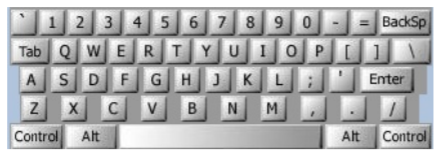
\includegraphics[width=\textwidth]{UVa10082}

\begin{flushleft}
{\color{red} \textbf{Input}}
\end{flushleft}
Input cosists of several lines of text. Each line may contain digits, spaces, upper case letter (except \textbf{Q}, \textbf{A}, \textbf{Z}), or punctuation shown above [except back-quote (\textbf{`})]. Keys labelled with words[\textbf{Tab}, \textbf{BackSp}, \textbf{Contral}, etc.] are not represented in the input.

\begin{flushleft}
{\color{red} \textbf{Output}}
\end{flushleft}
You are to replace each letter or punction symbol by the one immediately to its left on the \textbf{'QWERTY'} keyboard shown above. Spaces in the input should be echoed in the output.

\begin{flushleft}
{\color{red} \textbf{Sample Input}}
\end{flushleft}
\begin{flushleft}
O S, GOMR YPFSU/\\
\end{flushleft}

\begin{flushleft}
{\color{red} \textbf{Sample Output}}
\end{flushleft}
\begin{flushleft}
I AM FINE TODAY.
\end{flushleft}

\newpage